\documentclass[11pt,a4paper, german, english, swedish
]{article}
\pdfoutput=1

\usepackage{custom_as}

\graphicspath{ {figurer/} }

%%Drar in tabell och figurtexter
\usepackage[margin=10 pt]{caption}
%%För att lägga in 'att göra'-noteringar i texten
\usepackage{todonotes} %\todo{...}

%%För att själv bestämma marginalerna. 
\usepackage[
%            top    = 3cm,
%            bottom = 3cm,
%            left   = 3cm, right  = 3cm
]{geometry}

%%För att ändra hur rubrikerna ska formateras
%\renewcommand{\thesection}{...}


\newcommand{\BM}{\ifmmode\upbeta^{-}\else$\upbeta^{-}$\fi}
\newcommand{\BP}{\ifmmode\upbeta^{+}\else$\upbeta^{+}$\fi}
\newcommand{\G}{\ifmmode\upgamma\else$\upgamma$\fi}
\newcommand{\Thalv}{\ifmmode{T_{\nicefrac{1}{2}}}\else$T_{\nicefrac{1}{2}}$\fi}

\begin{document}



%%%%%%%%%%%%%%%%% vvv Inbyggd titelsida vvv %%%%%%%%%%%%%%%%%

\title{ Isotopproduktion för PET: \\[1mm] \Large Räkneuppgift nr.\,10, subatomär fysik}
\author{Andréas Sundström}
\date{\today}

\maketitle

%%%%%%%%%%%%%%%%% ^^^ Inbyggd titelsida ^^^ %%%%%%%%%%%%%%%%%


\section{Inledning}
Innan Röntgens upptäckt 1895\cite{Roentgen1895} av den strålning som nu är uppkallade efter honom, röntgenstrålar, har det enda sättet att undersöka människokroppens inre varit att skära upp den. Men även röntgenstrålning har sina baksidor. Exempelvis kan man bara se täta och hårda strukturer så som ben med dem. Det har därför med åren utvecklats fler tekniker för att skåda in i kroppen. 

En av dessa tekniker är \emph{positronemissionstomografi} (PET)\cite{Sweet&Brownell1955,Phelps_etal1975}. Den bygger på att en radioisotop som sönderfaller med \BP-sönderfall kan lokaliseras i kroppen genom att detektera koincidenta \G-strålar från elektron-positronanhileringen. För att detta ska kunna användas medicinskt krävs även att radioisotopen i fråga kan ansamlas i exempelvis tumörer som man vill undersöka.

I nuläget är PET-skanning en etablerad metod runt om i värdens sjukhus. Eftersom man vill ha tillräckligt hög strålningsintensitet vid skanningstillfället, men samtidigt inte vara för länge efteråt, så används oftast isotoper med relativt korta halveringstider. Detta betyder att sjukhusen behöver ha egna cyklotroner för isotopproduktion.

\subsubsection*{Specifikationer}
I den här rapporten beskrivs hur man kan gå tillväga, ur ett fysiklaiskt perspektiv, för att välja ut och förbereda en sådan radioisotop. Det finns två huvudsakliga delar här: att välja ut en lämplig isotop och hur produktionen ska dimensioneras.

Den cyklotron som används kan ge protoner med maximal energi på $E_\text{max}=\unit[10]{MeV}$ och ström på $I=\unit[10]{\micro{A}}$. Utgående från denna cyklotron, behövs en isotop med halveringstid på ungefär $\Thalv=\unit[17]{timmar}$. Självklart måste även isotopen \BP-sönderfalla för att kunna vara akutell för PET.

Produktionen ska sedan kunna vara stor nog för att kunna injecera fem patienter med ett antal av dessa kärnor motsvarande en strålningsintensitet på $A_\text{dos}=\unit[2.1]{MBq}$. Detta ska dessutom kunna göras efter att isotoperna har extraherats ur strålmålet som tar $t_0=\unit[54]{timmar}$ från avslutad betrålning. Samtidigt ska protonenergin inte vara så hög att det inte bildas några exciterade kärnor med högre än \unit[200]{keV} excitationsenergi. 



\section{Isotopval}
I National Nuclear Data Centers ''Nuclear Wallet Cards''\cite{NNDC_wallet} kan man specificera vilken typ av sönderfall och hur lång halveringstid man söker, så tar de fram de isotoper som matchar sökningen. Gör man en sökning efter \BP-sönderfallande isotoper med en halveringstid på $\unit[17\pm 1]{timmar}$ får man 12 möjliga kandidater. Av dessa har en av dem ($^{242}_{95}\!\mathrm{Am}$) bara en smal sönderfallskanal via \BP-sönderfall (17,30\,\%), så det är effektivt 11 möjliga isotoper att välja på.

Nästa steg i processen är att identifiera vilka isotoper som enkelt går att producera. Detta betyder de ska gå att producera genom protonbetråning på ett strålmål av naturligt förekommande isotoper\footnotemark{}. Av de 11~kandidaterna går det nu att sålla ut tre (3) med det här extrakravet. 
\footnotetext{Jag använder här den lista som är given på PingPong~\cite{PingPong}.}

De tre möjliga kandidaterna är: $^{55}_{27}\mathrm{Co}$, $^{76}_{35}\mathrm{Br}$ och $^{193}_{79}\!\mathrm{Au}$. Dessa kan nu slås upp i en nulkeidkarta~\cite{NNDC_chart}. Där kan man börja med att se att $^{193}_{79}\!\mathrm{Au}$ sönderfaller till $^{193}_{78}\mathrm{Pt}$, som också är radioaktiv med en halveringstid på 50~år. Detta är inte så bra. Man behöver visserligen en radioaktiv isotop för att kunna använda PET, men man vill ju heller inte att den ska lämna kvar rester som fortsätter att vara radioaktiva under en längre tid. Det visar sig även att $^{55}_{27}\mathrm{Co}$ har samma problem.

\subsubsection*{Den utvalda isotopen}
Då återstår bara $^{76}_{35}\mathrm{Br}$. Som tur är, så sönderfaller $^{76}_{35}\mathrm{Br}$ till $^{76}_{34}\mathrm{Se}$, som är stabil. Vidare är faktiskt $^{76}_{35}\mathrm{Br}$ en redan använd radioisotop för PET~\cite{Lapi_PET,Valette_etal1993,Lovqvist_etal1997,Ribeiro_etal1999}. Detta talar också för att det redan finns utvecklade metoder för att ge patienten isotopen medicinskt så att det går att upptäcka tumörer. 

Valet i det här fallet föll alltså på:
\[
^{76}_{35}\mathrm{Br}\qcomma 
\text{med } \Thalv=\unit[16,2]{timmar} \Longleftrightarrow \lambda = \unit[1,19\times10^{-5}]{s^{-1}}.
\]
Enligt \cite{PingPong} har $^{76}_{35}\mathrm{Br}$ en tröskelenergi på $E_\text{min}=\unit[5,8]{MeV}$, det är alltså görbart att producera isotopen med den givna cyklotronen.




\section{Produktion}
När isotopen väl är val måste produktionen av den dimensioneras.

\subsection{Mängd som behöver produceras}

Eftersom preparaten behöver förberedas i $t_0=\unit[54]{timmar}$ efter att produktionen avslutas, måste man ta hänsyn till att radioisotopen sönderfaller under tiden. Dett sker enligt den välkända exponenitellt avtagande kurvan
\begin{equation}
N_\text{s}(t) = N_0\,\ee^{-\lambda t}, %= N_0\cdot 2^{-t/\Thalv}
\end{equation}
där $N_\text{s}$ är antalet kärnor som finns vid tiden $t$, $N_0$ antalet kärnor som kommer från produktionen och $\lambda$ är radioisotopens sönderfallskonstant. I det här fallet är $t_0\approx3\Thalv$, vilket innebär att bara ungefär en åttondel av de producerade kärnorna har överlevt när patienten får dem. 

PET-skanner kräver att patienterna får en dos på $A_\text{dos}=\unit[2.1]{MBq}$ -- dosen ska ges till fem patienter samtidigt. Eftersom aktiviteten följer
\begin{equation}
A(t) = -\dv{N_\text{s}}{t} 
= \lambda N_0\,\ee^{-\lambda t}
\end{equation}
bestämmer detta hur många kärnor som måste produceras. 

Man måste helt enkelt komma upp i $\lambda N_0\,\ee^{-\lambda t_0} = 5A_\text{dos}$. Detta ger en ekvation för för hur många kärnor som måste produceras i cyklotronen:
\begin{equation}
N_0 = \frac{5}{\lambda}\,A_\text{dos}\ee^{\lambda t_0} 
= \frac{5}{\ln{2}}\,\Thalv\,A_\text{dos}\cdot 2^{t_0/\Thalv}
= \unit[8,90\times 10^{12}]{kärnor}.
\end{equation}


\subsection{Cyklotronen}
När antalet radioaktiva kärnor som behöver produceras väl är bestämt måste själva produktionen dimensioneras. Antalet radioaktiva kärnor som finns efter tiden $t$ från starten av produktionen är
\begin{equation}
N_\text{p}(t) = \frac{R}{\lambda} \left( 1-\ee^{-\lambda t} \right),
% = \frac{R}{\lambda} \left( 1-2^{-t/\Thalv} \right)
\end{equation}
där $R$ är produktionstakten definierad enligt
\begin{equation}
R=\sigma n I,
\end{equation}
där $\sigma$ är reaktionens tvärsnitt, $I$ är strålens intensitet (i protoner per sekund) och $n$ är strålmålstätheten (i strålmålskärnor per längdenhet). I det här fallet är intensiteten given i ampere. För att konvertera till protoner per sekund används $I=i/e$. 
Det sammanlagda uttrycket blir alltså
\begin{equation}
N_\text{p}(t) = \frac{\sigma n i}{\lambda e} \left( 1-\ee^{-\lambda t} \right).
\end{equation}

\todo[inline]{Bla bla problem med andra isotoper som produceras vilket ger \G-strålning med för hög energi.}


\begin{figure}\centering
% GNUPLOT: LaTeX picture with Postscript
\begingroup
  \makeatletter
  \providecommand\color[2][]{%
    \GenericError{(gnuplot) \space\space\space\@spaces}{%
      Package color not loaded in conjunction with
      terminal option `colourtext'%
    }{See the gnuplot documentation for explanation.%
    }{Either use 'blacktext' in gnuplot or load the package
      color.sty in LaTeX.}%
    \renewcommand\color[2][]{}%
  }%
  \providecommand\includegraphics[2][]{%
    \GenericError{(gnuplot) \space\space\space\@spaces}{%
      Package graphicx or graphics not loaded%
    }{See the gnuplot documentation for explanation.%
    }{The gnuplot epslatex terminal needs graphicx.sty or graphics.sty.}%
    \renewcommand\includegraphics[2][]{}%
  }%
  \providecommand\rotatebox[2]{#2}%
  \@ifundefined{ifGPcolor}{%
    \newif\ifGPcolor
    \GPcolortrue
  }{}%
  \@ifundefined{ifGPblacktext}{%
    \newif\ifGPblacktext
    \GPblacktexttrue
  }{}%
  % define a \g@addto@macro without @ in the name:
  \let\gplgaddtomacro\g@addto@macro
  % define empty templates for all commands taking text:
  \gdef\gplbacktext{}%
  \gdef\gplfronttext{}%
  \makeatother
  \ifGPblacktext
    % no textcolor at all
    \def\colorrgb#1{}%
    \def\colorgray#1{}%
  \else
    % gray or color?
    \ifGPcolor
      \def\colorrgb#1{\color[rgb]{#1}}%
      \def\colorgray#1{\color[gray]{#1}}%
      \expandafter\def\csname LTw\endcsname{\color{white}}%
      \expandafter\def\csname LTb\endcsname{\color{black}}%
      \expandafter\def\csname LTa\endcsname{\color{black}}%
      \expandafter\def\csname LT0\endcsname{\color[rgb]{1,0,0}}%
      \expandafter\def\csname LT1\endcsname{\color[rgb]{0,1,0}}%
      \expandafter\def\csname LT2\endcsname{\color[rgb]{0,0,1}}%
      \expandafter\def\csname LT3\endcsname{\color[rgb]{1,0,1}}%
      \expandafter\def\csname LT4\endcsname{\color[rgb]{0,1,1}}%
      \expandafter\def\csname LT5\endcsname{\color[rgb]{1,1,0}}%
      \expandafter\def\csname LT6\endcsname{\color[rgb]{0,0,0}}%
      \expandafter\def\csname LT7\endcsname{\color[rgb]{1,0.3,0}}%
      \expandafter\def\csname LT8\endcsname{\color[rgb]{0.5,0.5,0.5}}%
    \else
      % gray
      \def\colorrgb#1{\color{black}}%
      \def\colorgray#1{\color[gray]{#1}}%
      \expandafter\def\csname LTw\endcsname{\color{white}}%
      \expandafter\def\csname LTb\endcsname{\color{black}}%
      \expandafter\def\csname LTa\endcsname{\color{black}}%
      \expandafter\def\csname LT0\endcsname{\color{black}}%
      \expandafter\def\csname LT1\endcsname{\color{black}}%
      \expandafter\def\csname LT2\endcsname{\color{black}}%
      \expandafter\def\csname LT3\endcsname{\color{black}}%
      \expandafter\def\csname LT4\endcsname{\color{black}}%
      \expandafter\def\csname LT5\endcsname{\color{black}}%
      \expandafter\def\csname LT6\endcsname{\color{black}}%
      \expandafter\def\csname LT7\endcsname{\color{black}}%
      \expandafter\def\csname LT8\endcsname{\color{black}}%
    \fi
  \fi
  \setlength{\unitlength}{0.0500bp}%
  \begin{picture}(6802.00,3968.00)%
    \gplgaddtomacro\gplbacktext{%
      \csname LTb\endcsname%
      \put(860,640){\makebox(0,0)[r]{\strut{} 0}}%
      \csname LTb\endcsname%
      \put(860,1081){\makebox(0,0)[r]{\strut{} 100}}%
      \csname LTb\endcsname%
      \put(860,1522){\makebox(0,0)[r]{\strut{} 200}}%
      \csname LTb\endcsname%
      \put(860,1963){\makebox(0,0)[r]{\strut{} 300}}%
      \csname LTb\endcsname%
      \put(860,2404){\makebox(0,0)[r]{\strut{} 400}}%
      \csname LTb\endcsname%
      \put(860,2845){\makebox(0,0)[r]{\strut{} 500}}%
      \csname LTb\endcsname%
      \put(860,3286){\makebox(0,0)[r]{\strut{} 600}}%
      \csname LTb\endcsname%
      \put(860,3727){\makebox(0,0)[r]{\strut{} 700}}%
      \csname LTb\endcsname%
      \put(980,440){\makebox(0,0){\strut{} 5}}%
      \csname LTb\endcsname%
      \put(2072,440){\makebox(0,0){\strut{} 6}}%
      \csname LTb\endcsname%
      \put(3164,440){\makebox(0,0){\strut{} 7}}%
      \csname LTb\endcsname%
      \put(4257,440){\makebox(0,0){\strut{} 8}}%
      \csname LTb\endcsname%
      \put(5349,440){\makebox(0,0){\strut{} 9}}%
      \csname LTb\endcsname%
      \put(6441,440){\makebox(0,0){\strut{} 10}}%
      \put(160,2183){\rotatebox{-270}{\makebox(0,0){\strut{}$\sigma$ /[b]}}}%
      \put(3710,140){\makebox(0,0){\strut{}$E$ /[MeV]}}%
    }%
    \gplgaddtomacro\gplfronttext{%
      \csname LTb\endcsname%
      \put(1580,3484){\makebox(0,0)[r]{\strut{}$^{76}_{34}\mathrm{Se}$}}%
    }%
    \gplbacktext
    \put(0,0){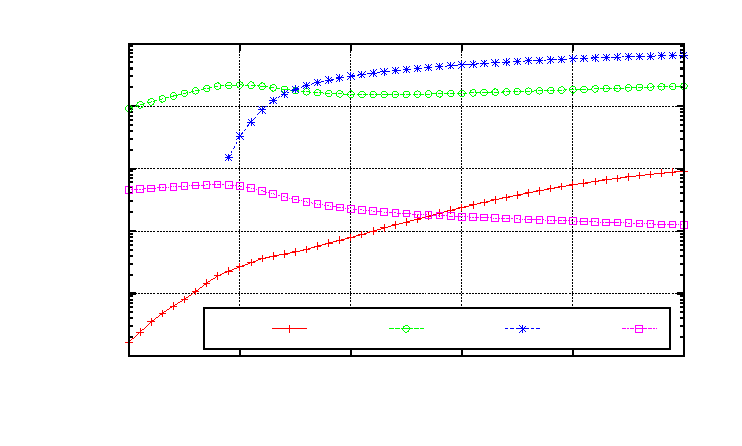
\includegraphics{Se_76_x-sect}}%
    \gplfronttext
  \end{picture}%
\endgroup

\caption{Simulerat~\cite{PingPong} tvärsnitt för isotopproduktion med protonstråle med $^{76}_{34}\mathrm{Se}$ som strålmål. Det finns fyra möjliga raktionsprodukter utmarkerade, varav $^{76}_{35}\mathrm{Br}$ är den eftersökta isotopen. }
\label{fig:x-sect}
\end{figure}



\section{Sammanfattning}



%\newpage
\bibliographystyle{ieeetr}
\bibliography{referenser}%kräver en fil som heter 'referenser.bib'          



\end{document}





%% På svenska ska citattecknet vara samma i både början och slut.
%% Använd två apostrofer (två enkelfjongar): ''.


%% Inkludera PDF-dokument
\includepdf[pages={1-}]{filnamn.pdf} %Filnamnet får INTE innehålla 'mellanslag'!

%% Figurer inkluderade som pdf-filer
\begin{figure}\centering
\centerline{ %centrerar även större bilder
\includegraphics[width=1\textwidth]{filnamn.pdf}
}
\caption{}
\label{fig:}
\end{figure}

%% Figurer inkluderade med xfigs "Combined PDF/LaTeX"
\begin{figure}\centering
\resizebox{.8\textwidth}{!}{\input{filnamn.pdf_t}}
\caption{}
\label{fig:}
\end{figure}

%% Figurer roterade 90 grader
\begin{sidewaysfigure}\centering
\centerline{ %centrerar även större bilder
\includegraphics[width=1\textwidth]{filnamn.pdf}
}
\caption{}
\label{fig:}
\end{sidewaysfigure}


%%Om man vill lägga till något i TOC
\stepcounter{section} %Till exempel en 'section'
\addcontentsline{toc}{section}{\Alph{section}\hspace{8 pt}Labblogg} 

